\documentclass[12pt]{article}
\usepackage{tikz}
\usepgflibrary{arrows}

\begin{document}
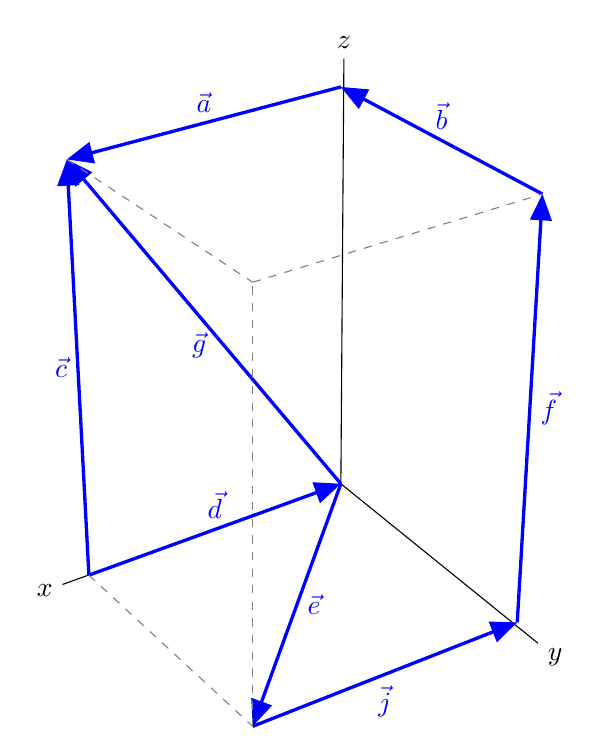
\begin{tikzpicture}[scale=4,>=triangle 45]
  \node (C) at (0.81, 0.87) {}; % origin
%  \node (X) at (1.69, 0.55) {$x$}; % x-axis
%  \node (Y) at (0.18, 0.38) {$y$}; % y-axis
%  \node (Z) at (0.79, 2.27) {$z$}; % z-axis
  \node (X) at (0.11, 0.52) {$x$};
  \node (Y) at (1.73, 0.31) {$y$};
  \node (Z) at (1.06, 2.26) {$z$};
  \draw (1.05, 0.86) -- (X);
  \draw (1.05, 0.86) -- (Y);
  \draw (1.05, 0.86) -- (Z);
  \draw[->,very thick,blue] (1.05, 2.12) -- node[above] {$\vec{a}$} (0.18, 1.89);
  \draw[->,very thick,blue] (1.69, 1.78) -- node[above] {$\vec{b}$} (1.05, 2.12);
  \draw[->,very thick,blue] (0.25, 0.57) -- node[left]  {$\vec{c}$} (0.18, 1.89);
  \draw[->,very thick,blue] (0.25, 0.57) -- node[above] {$\vec{d}$} (1.05, 0.86); 
  \draw[->,very thick,blue] (1.05, 0.86) -- node[right] {$\vec{e}$} (0.77, 0.09);
  \draw[->,very thick,blue] (1.61, 0.42) -- node[right] {$\vec{f}$} (1.69, 1.78);
  \draw[->,very thick,blue] (1.05, 0.86) -- node[below] {$\vec{g}~$} (0.18, 1.89);
  \draw[->,very thick,blue] (0.77, 0.09) -- node[below] {$\vec{j}$} (1.61, 0.42);
  \draw[dashed,gray] (0.25, 0.57) -- (0.77, 0.09);
  \draw[dashed,gray] (0.77, 0.09) -- (0.77, 1.50); 
  \draw[dashed,gray] (0.18, 1.89) -- (0.77, 1.50);
  \draw[dashed,gray] (0.77, 1.50) -- (1.69, 1.78);
\end{tikzpicture}
\end{document}